\chapter{Activiti BPM}\label{chp:activiti}

\section{Introdução}\label{sec:activiti-introducao}
Criado em 2010 por ex-integrantes do projeto jBPM, o Activiti BPM é um projeto de código aberto sob a licença Apache V2, que provê um motor BPM leve e completo sob a especificação BPMN 2.0. O Activiti é desenvolvido sob a linguagem de programação Java e é facilmente integrável com aplicações existentes por sua leveza e API amigável.

Neste capítulo vamos apresentar como o Activiti BPM pode ser utilizado na automatização de processos de negócio. Vamos apresentar ainda, a capacidade de modelagem de processos através da notação BPMN utilizada pelo Activiti. Por último vamos abordar as vantagens e limitações desta ferramenta frente às demais opções do mercado.

\section{BPMN}\label{sec:activiti-bpmn}
A BPMN (Business Process Management Notation) foi criada para representar processos de negócio em forma de diagrama, através de uma notação padronizada e de fácil entendimento por diferentes profissionais, sejam desenvolvedores, analistas de negócio ou gestores. Foi criada inicialmente pelo BPMI (Business Process Management Initiative) em 2004, mas atualmente é mantida e atualizada pela OMG (Object Management Group). Sua versão mais atual é a BPMN 2.0, publicada em 2011.

A notação foi concebida sob a perspectiva de cobrir a falta de entendimento entre diferentes departamentos e organizações a cerca de um determinado processo ou conjunto de processos, algo muito frequente no ambiente corporativo. Além disso, através de sua notação padronizada em XML (Extensible Markup Language), diferentes ferramentas podem fazer o uso de sua auto-descrição para orquestração de processos de negócio, sejam eles automatizáveis ou não.

A notação define quatro grupos distintos de objetos para permitir a diagramação de um fluxo de negócio. Os objetos são classificados em artefatos, agrupadores, conectores e objetos de fluxo. São utilizadas figuras geométricas, como retângulos e círculos, além de linhas pontilhadas e tracejadas, entre outros elementos para representar cada um dos objetos que constituem a notação.

1) http://searchcio.techtarget.com/definition/Business-Process-Modeling-Notation

2) http://blog.iprocess.com.br/2012/11/um-guia-para-iniciar-estudos-em-bpmn-i-atividades-e-sequencia

3) https://www.fluig.com/blog/entendendo-melhor-o-bpmn/

\begin{figure}
  \centering
  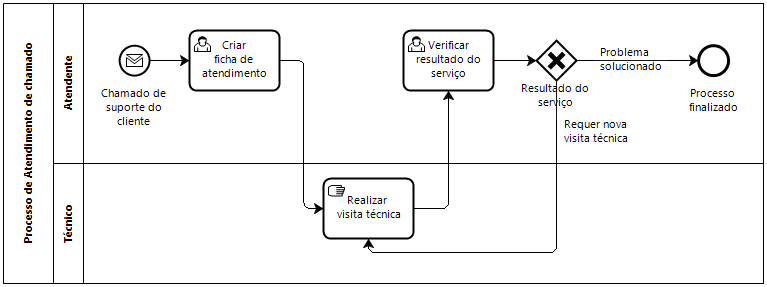
\includegraphics[width=1.0\textwidth]{imagens/bpmn_example.png}
  \caption{Exemplo de processo representado em BPMN}
  \label{fig:exemplo_bpmn}
\end{figure}

\section{Gestão de processos com o Activiti BPM}\label{sec:activiti-gestao_processos}

O Activiti é constituído através de diversos componentes que juntos possibilitam o aproveitamento do ecossistema BPM. Com exceção do Activiti Engine, pois este constitui o módulo principal da ferramenta, todos os demais módulos são opcionais e dependem do cenário de utilização da ferramenta.

O Activiti Engine é o componente principal, pois nele estão presentes o motor de funcionamento do BPM e as APIs para acesso e controle da ferramenta. Este componente é disponibilizado através de um simples arquivo JAR, modelo de arquivo padrão para bibliotecas da linguaguem Java. Sendo assim, o motor BPM pode ser facilmente utilizado em diferentes projetos Java através da inclusão dessa biblioteca como dependência.

Além da API Java, que está incluída no motor BPM, o Activiti REST API disponibiliza um acesso às funcionalidades principais do Activiti através de uma interface REST. Isso simplifica o acesso às suas funcionalidades e facilita a construção das mais variadas aplicações de interface com o usuário, como por exemplo, aplicações móveis.

O Activiti Designer, é um plugin criado para a interface de desenvolvimento Eclipse, que permite ao analista ou desenvolvedor modelar processos na notação BPMN graficamente, ao mesmo tempo em que é gerado automaticamente a notação do processo em XML.

O Activiti Explorer é a interface web padrão com o usuário, disponibilizada para o controle e execução de processos. Através dessa interface, o usuário pode instalar novas definições de processos, iniciar ou cancelar processos, finalizar ou delegar tarefas.

O Activiti exige um ambiente Java JDK versão 6 ou superior para seu correto funcionamento. Além do ambiente Java configurado, também é necessário um banco de dados para suportar a persistência das informações dos processos. Uma variedade de bancos é suportada pelo BPMS, são eles: H2, MySQL, Oracle, Postgres, DB2 e SQL Server.

\section{Como automatizar um processo?}\label{sec:activiti-automatizar_processo}

Nesta seção, iremos detalhar uma abordagem simplificada, porém suficiente para ilustrar os passos necessários para a automatização de um processo de negócio na ferramenta.  O processo de negócio utilizado como base é o mesmo apresentado na seção de introdução deste trabalho.

\subsection{Configuração do Ambiente}\label{sec:activiti-automatizar_processo_configuracao_ambiente}

O primeiro passo necessário é a preparação do ambiente de execução do BPM. Para isso, existem duas possibilidades principais. A primeira opção é a inclusão da dependência do Activiti BPM em um projeto Java web específico, e posterior construção do pacote WAR para execução em um servidor Java web. Outra opção, mais simples e que será utilizada nesta seção, é a utilização de um pacote WAR pronto para funcionamento (activiti-explorer.war), disponibilizado diretamente no site da ferramenta (www.activiti.org).

O arquivo disponibilizado no portal da ferramenta já inclui o Activiti Engine e o Activiti Explorer num único pacote, pré-configurados com um banco de dados em memória H2 que dá suporte ao seu funcionamento e não requer nenhuma configuração adicional. Para iniciar a execução do BPMS, basta a instalação do artefato em um servidor Java web como o Apache Tomcat 7 que será utilizado neste trabalho.

Após a instalação do artefato e inicialização do Tomcat, o portal pode ser acessado através do endereço http://127.0.0.1:8080/activiti-explorer, dado que o Tomcat tenha sido instalado na sua configuração padrão. O usuário e senha padrão para acesso ao portal como administrador é kermit.



\section{Vantagens e Limitações}\label{sec:activiti-vantages_limitacoes}


